\part{Предисловие}

Между школьной и университетской математиками существует категорическое
различие: в школе математику рассматривают как определённый ``закон природы'',
то есть $1+1=2$ потому что это так. В университете же математику изучают
в рамках формальной системы с чётко определёнными правилами.

\textsc{Университетская математика вводит аксиомы, из которых выводит теоремы,
  в отличие от школьной математики, которая
  в основном строится на интуитивных рассуждениях.}

Данная книга стремится доступно и точно сформулировать понятия аксиомы,
теоремы, доказательства и дать необходимый фундамент для построения
интуитивного понимания математических формул.

В тексте достаточно много сносок, они содержат важные оговорки,
улучшающие понимание материала. В качестве практики
после некоторых глав предложены упражнения. Упражнения с повышенной сложностью
отмечены~*.
По всем вопросам обращайтесь по адресу {\sl kksenya758@gmail.com}.

\part{Основные понятия}

\section{Формулы и выражения}

Математика обращается с высказываниями о математических объектах.
Рассмотрим структуру высказываний в человеческом языке.
Высказывания можно объединять с помощью
союзов. Например, высказывания ``небо синее''
и ``трава зелёная'' можно союзом ``и'' объединить в высказывание
``небо синее и трава зелёная''. Более сложное высказывание с несколькими
логическими союзами можно представить в виде дерева:

\vspace{-1.25em}
\begin{center}
  \begin{tikzpicture}
    \node (m) at (0,0) {Если все люди смертны и Сократ --- человек,
      то Сократ смертен.};
    \node (l) at (-2,-1) {Все люди смертны и Сократ --- человек};
    \node (r) at (3.5,-1) {Сократ смертен};
    \node (ll) at (-4,-2) {Все люди смертны};
    \node (lr) at (0,-2) {Сократ --- человек};

    \draw (m) -- (l) -- (ll);
    \draw (m) -- (r);
    \draw (l) -- (lr);
  \end{tikzpicture}
\end{center}

\vspace{-0.25em}
\index{высказывание!сложное}\index{высказывание!элементарное}
\index{сложное!высказывание}\index{элементарное!высказывание}
Высказывание, которое может быть построено из других высказываний с помощью
союзов, называют {\it сложным высказыванием}.
Высказывание, которое не является сложным, называют {\it элементарным}.
По определению сложное высказывание можно разложить в дерево до
элементарных высказываний.

\index{алфавит}
Человеческий язык достаточно неточен, поэтому создадим более точный язык формул.
{\it Алфавитом} будем называть совокупность знаков\footnote{
  Используется слово ``знак'', а не ``символ'', потому что некоторые знаки
  состоят из нескольких символов. Например, $x_1$, $x_2$.} этого языка.
Его можно разделить на четыре части:
\begin{enumerate}
  \item{}{\it Знаки переменных}\index{знак!переменной} --- буквы латинского,
  греческого и других алфавитов с индексами, различными значками и без.

  Например, $x,y,z,z_1,x_2,\hat x,a'$.

  \item{}{\it Знаки функций и отношений}\index{знак!функций и отношений}
  --- знаки, обозначающие
  различиные функции ($\sin$, $+$) и отношения ($=$, $\leq$, $\in$).

  \item{}{\it Союзы}\index{союз}
  --- знаки ``и'', ``или'', следстивия и прочие.

  \item{}{\it Знаки препинания}\index{знак!препинания} --- скобки,
  запятые, двоеточия и прочие.
\end{enumerate}

{\it Выражение}\index{выражение} --- любая последовательность знаков алфавита.
Выражение не обязательно имеет смысл, но определённым выражениям мы его придаём,
интерпретируя их.

Обращаясь с выражениями, удобно использовать сокращения. Запись
$\varphi\equiv a_1a_2...a_{n}$ означает, что за сокращением $\varphi$
стоит выражение $a_1a_2...a_{n}$, где $a_1,...,a_{n}$ --- знаки алфавита.
Если ${\varphi\equiv a_1...a_{n}}$ и ${\psi\equiv b_1...b_{m}}$,
то $\varphi\psi\equiv a_1...a_{n}b_1...b_{m}$. То есть
за сокращением $\varphi\psi$ стоит выражение $a_1...a_{n}b_1...b_{m}$.

  {\it Формула}\index{формула} --- выражение,
соответсвующее определённому утверждению, высказыванию
(например, $2+2=5$). 
\begin{marginfigure}[3.5cm]
  \centering
  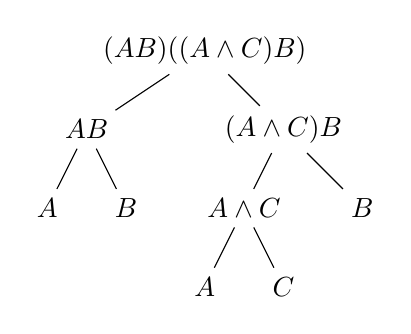
\begin{tikzpicture}
    \node (main) at (0,0) {$(A\implies B)\implies ((A\land C)\implies B)$};
    \node (l) at (-1.5,-1) {$A \implies B$};
    \node (r) at (1,-1) {$(A\land C)\implies B$};
    \node (ll) at (-2,-2) {$A$};
    \node (lr) at (-1,-2) {$B$};
    \node (rl) at (0.5,-2) {$A\land C$};
    \node (rr) at (2,-2) {$B$};
    \node (rll) at (0,-3) {$A$};
    \node (rlr) at (1,-3) {$C$};

    \draw (main) -- (l);
    \draw (main) -- (r);
    \draw (l) -- (ll);
    \draw (l) -- (lr);
    \draw (r) -- (rl);
    \draw (r) -- (rr);
    \draw (rl) -- (rll);
    \draw (rl) -- (rlr);
  \end{tikzpicture}

  \caption{Дерево формулы}\label{fig:form_tree}
\end{marginfigure}

\index{элементарное!формула}\index{формула!элементарная}
Введём в алфавит союзы $\lnot$, $\land$, $\lor$, $\implies$, $\iff$
и знаки $\top$, $\bot$.
Позже определим, каким союзам и высказываниям в человеческом
языке они соотвествуют.

Будем называть $\top$ и $\bot$ {\it элементарными формулами}.
Определим, какие выражения будем считать формулами (какие выражения 
будем интерпретировать как высказывания).
\begin{enumerate}
  \item{}Любая элементарная формула --- формула.

  \item{}Если выражения $A,B$ --- формулы\footnote{То есть за 
      сокращениями $A$ и $B$ стоят выражения, которые являются 
      формулами.}, то выражения
  \begin{equation}\label{eq:comp_formulas}
    \lnot A\qquad A\land B\qquad A\lor B\qquad A\implies B\qquad A\iff B
  \end{equation}
  также являются формулами.
\end{enumerate}

\begin{marginfigure}[0.75cm]
  \centering
  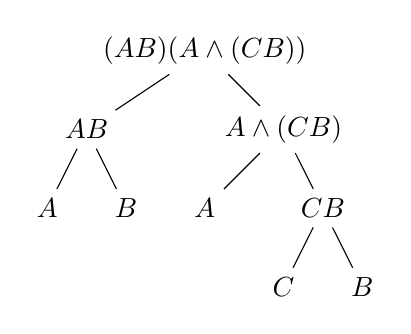
\begin{tikzpicture}
    \node (main) at (0,0) {$(A\implies B)\implies (A\land (C\implies B))$};
    \node (l) at (-1.5,-1) {$A \implies B$};
    \node (r) at (1,-1) {$A\land (C\implies B)$};
    \node (ll) at (-2,-2) {$A$};
    \node (lr) at (-1,-2) {$B$};
    \node (rl) at (0,-2) {$A$};
    \node (rr) at (1.5,-2) {$C\implies B$};
    \node (rrl) at (1,-3) {$C$};
    \node (rrr) at (2,-3) {$B$};

    \draw (main) -- (l);
    \draw (main) -- (r);
    \draw (l) -- (ll);
    \draw (l) -- (lr);
    \draw (r) -- (rl);
    \draw (r) -- (rr);
    \draw (rr) -- (rrl);
    \draw (rr) -- (rrr);
  \end{tikzpicture}

  \caption{Дерево формулы с другими скобками}\label{fig:form_tree_2}
\end{marginfigure}

\index{сложное!формула}\index{формула!сложная}
\index{подформула}
По аналогии с высказываниями, формулы \eqref{eq:comp_formulas}
называют {\it сложными}.
Формулы, из которых была построена сложная формула
называют её {\it подформулами}.

Точно так же, как и сложное высказывание, сложную формулу можно
разложить в дерево (рис.~\ref{fig:form_tree}). Причём скобки будут
определять, по какому союзу должно идти разложение (рис.~\ref{fig:form_tree_2}).
В этих двух примерах $A,B,C$ и $A\implies B$ являются подформулами.

Как и сложное высказывание, чтобы понять сложную формулу
необходимо знать, в каком порядке она была построена из своих подформул.
Однако формулу $A\implies B\land C$ можно разложить на $A,B,C$ двумя
способами (рис.~\ref{fig:amb_form}).
Поэтому определяют правила, по которым каждой сложной формуле
соотвествует единственное дерево, а значит и единственный союз,
по которому формулу можно разложить.
Например, можно определить порядок союзов и разлагать формулу по первому
подходящему союзу в порядке.

\begin{marginfigure}[-2cm]
  \begin{multicols}{2}
    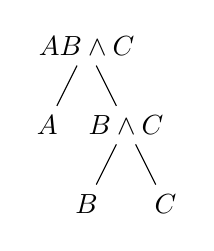
\begin{tikzpicture}
      \node (m) at (0,0) {$A\implies B\land C$};
      \node (l) at (-0.5,-1) {$A$};
      \node (r) at (0.5,-1) {$B\land C$};
      \node (rl) at (0,-2) {$B$};
      \node (rr) at (1,-2) {$C$};

      \draw (m) -- (r) -- (rr);
      \draw (m) -- (l);
      \draw (r) -- (rl);
    \end{tikzpicture}

    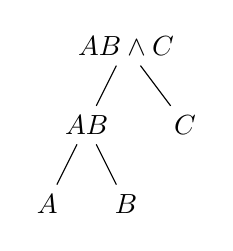
\begin{tikzpicture}
      \node (m) at (0,0) {$A\implies B\land C$};
      \node (l) at (-0.5,-1) {$A\implies B$};
      \node (r) at (0.75,-1) {$C$};
      \node (ll) at (-1,-2) {$A$};
      \node (lr) at (0,-2) {$B$};

      \draw (m) -- (l) -- (ll);
      \draw (l) -- (lr);
      \draw (m) -- (r);
    \end{tikzpicture}
  \end{multicols}

  \caption{Варианты разложения формулы}\label{fig:amb_form}
\end{marginfigure}

Определим следующий порядок:
\begin{enumerate}
  \item{}$\implies$ или $\iff$. Выражения вида ${A\implies B\implies C}$
  будем рассматривать по-другому.
  \item{}Самый правый $\lor$. 
    То есть $A\lor B \lor C$ разлагаем на $A\lor B$ и $C$.
  \item{}Самый правый $\land$.
  \item{}Самый левый $\lnot$.
\end{enumerate}

Далее будем рассматривать только формулы, которые по этим правилам можно
единственным образом разложить в дерево. Причём будем считать, что
обозначение $A\land B$ подразумевает, что скобки расставлены так,
чтобы $A\land B$ можно
было разложить только по $\land$ в подформулы $A$ и $B$. Аналогично будем рассматривать
такие обозначения с прочими союзами.
На рис.~\ref{fig:rules_tree} представлен пример использования правил
разложения формулы.

\begin{marginfigure}[-5cm]
  \centering
  \begin{tikzpicture}
    \node (m) at (0,0) {$A\implies A\lor\lnot A$};
    \node (ml) at (-1,-1) {$A$};
    \node (mr) at (1,-1) {$A\lor \lnot A$};
    \node (mrl) at (0,-2) {$A$};
    \node (mrr) at (2,-2) {$\lnot A$};
    \node (mrrm) at (2,-3) {$A$};

    \draw (m) -- (mr) -- (mrr) -- (mrrm);
    \draw (m) -- (ml);
    \draw (mr) -- (mrl);
  \end{tikzpicture}

  \caption{Разложение формулы без скобок.}\label{fig:rules_tree}
\end{marginfigure}

Формулы соответствуют утверждениям, высказываниям,
поэтому можно говорить об их {\it истинности}\index{истинность}.
Определим формулу $\top$ как истинную\footnote{Формула $\top$ истинна по определению,
поэтому знак $\top$ называют {\it знаком элементарной тавтологии}.
\index{знак!элементарного!тавтологии}\index{тавтология!элементарная}},
а $\bot$ как ложную\index{ложь} (не истинную).

Определим теперь, каким высказываниям соотвествуют сложные формулы.
Вместе с этим мы сформулируем правила определения истинностей сложных формул.
\begin{enumerate}
  \item{}И ($\land$)\index{и, $\land$}.
  $p\land q$ соотвествует высказыванию ``$p$ и $q$ истинны''.

  То есть $p\land q$ истинна, если $p$ и $q$ истинны,
  и ложна иначе. Обычно слова ``$A$ истинна'' сокращают до ``$A$''.

  \item{}Или ($\lor$)\index{или, $\land$}.
  $p\lor q$ соотвествует ``$p$ или $q$''.

  \item{}Отрицание ($\lnot$)\index{отрицание, $\lnot$}.
  $\lnot p$ соотвествует ``не $p$''.

  \item{}Следствие\index{следствие, $\implies$},
  импиликация\index{импиликация, $\implies$} ($\implies$).

  ${p\implies q}$ соотвествует ``для $q$ достаточно $p$''.
  % То есть всякий раз, когда $p$ истинно,
  % обязательно (необходимо) истинно и $q$.

  \textsc{Математическое следствие не подразумевает
    причинность}. Например, если $q$ истинно,
  то для $q$ будет достаточно $p$, где $p$ --- любая формула,
  ведь $q$ и так истинно.
  На языке формул это можно записать как $q\implies (p\implies q)$.

  \item{}Равносильность\index{равносильность, $\iff$},
  эквивалентность\index{эквивалентность, $\iff$} ($\iff$).

  $p\iff q$ соотвествует ``$p$ тогда и только тогда, когда $q$''.
\end{enumerate}

\begin{margintable}[7cm]
  \begin{tabular}{cl}
    $p\land q$    & $p$ и $q$                                   \\\hline
    $p\lor q$     & $p$ или $q$                                 \\\hline
    $\lnot p$     & не $p$                                      \\
                  & $p$ ложно                                   \\ \hline
    $p\implies q$ & если $p$, то $q$                            \\
                  & из $p$ следует $q$                          \\
                  & для $q$ достаточно\index{достаточность} $p$ \\
                  & для $p$ необходимо\index{необходимость} $q$ \\
                  & $q$ всякий раз, когда $p$                   \\\hline
    $p\iff q$     & $p$ эквивалентно $q$                        \\
                  & $p$ равносильно $q$                         \\
                  & $p\implies q$ и $q\implies p$               \\\hline
    $\top$        & истина                                      \\\hline
    $\bot$        & ложь                                        \\
                  & противоречие
  \end{tabular}

  \caption{Союзы}\label{table:read_form}
\end{margintable}

Другие варианты определений союзов можно
найти в таблице~\ref{table:read_form}.
Так, формула ${A\land B\implies C}$
соотвествует ``Для $C$ достаточно $A$ и $B$''.
Причём из-за неточности человеческого языка последнему
высказыванию может соотвествовать и
${(A\implies C)\land B}$.

\index{таблица истинности}
Истинность сложной формулы всегда можно определить, зная истинности
подформул. Для этого обычно пользуются {\it таблицой истинности} ниже.

\begin{center}
  \begin{tabular}{cc|ccccc}
    $p$    & $q$       & $p\land q$
           & $p\lor q$ & $\lnot p$  & $p\implies q$ & $p\iff q$                   \\\hline
    $\top$ & $\top$    & $\top$     & $\top$        & $\bot$    & $\top$ & $\top$ \\
    $\top$ & $\bot$    & $\bot$     & $\top$        & $\bot$    & $\bot$ & $\bot$ \\
    $\bot$ & $\top$    & $\bot$     & $\top$        & $\top$    & $\top$ & $\bot$ \\
    $\bot$ & $\bot$    & $\bot$     & $\bot$        & $\top$    & $\top$ & $\top$ \\
  \end{tabular}
\end{center}

Выражение из знаков переменных и знаков $\top$, $\bot$, $\land$, $\lor$, $\lnot$,
$\implies$ и $\iff$ называют
{\it простой тавтологией}\index{простая тавтология}\index{тавтология!простая}, если
% \begin{fullwidth}
%   \begin{multicols}{2}
\begin{enumerate}
  \item{}Оно является формулой, когда все знаки переменных в ней
  являются формулами.
  % \columnbreak
  \item{}Оно истинно при любых определённых истинностях формул знаков переменных.
\end{enumerate}
%   \end{multicols}
% \end{fullwidth}

Заметим, что проверить, является ли выражение простой тавтологией,
можно за конечное число шагов: достаточно просто перебрать все
возможные истинности формул знаков переменных.

Например, выражение ${(A\land (A\implies B))\implies B}$ --- формула,
когда $A,B$ --- формулы и
существует $4$ варианта определённых истинностей формул $A$ и $B$,
перебор которых можно организовать таблично (таблица~\ref{table:taut_check}).
Можем сделать вывод, что это выражение является простой тавтологией.
\begin{margintable}
  \begin{tabular}{cc|c}
    $A$    & $B$    & $F$    \\\hline
    $\top$ & $\top$ & $\top$ \\
    $\top$ & $\bot$ & $\top$ \\
    $\bot$ & $\top$ & $\top$ \\
    $\bot$ & $\bot$ & $\top$
  \end{tabular}

  \vspace{0.5em}
  $F\equiv{(A\land (A\implies B))\implies B}$

  \caption{Перебор истинностей $A$ и $B$}\label{table:taut_check}
\end{margintable}

Чтобы не путаться в круглых скобках, последнюю формулу можно записать используя
квадратные:
\[
  [A\land (A\implies B)]\implies B
\]
Квадратные скобки, как и круглые, могут быть использованы для определения порядка
разложения формулы.

\vspace{1em}
{\it Упражнения:}

\begin{enumerate}
  \item{}Показать, что следующие выражения --- простые тавтологии\label{ex:simple_taut}
  \begin{enumerate}
    \item{}$\top$
    \item{}$\lnot p\land p\iff\bot$\footnote{
    Знак $\bot$ по этой причине называют {\it знаком элементарного противоречия}.
    \index{знак!элементарного!противоречия}}
    \item{}$\bot \implies p$
    \item{}$p\land p\iff p$
    \item{}$p\implies (q\implies p)$
    \item{}$\lnot(p\lor q)\iff \lnot p\land \lnot q$
    --- закон Де Моргана\index{закон!Де Моргана}
    \item{}$p\lor \lnot p$ --- закон исключённого третьего
    \index{закон!исключённого третьего}
    \item{}${(p\implies q)\iff (\lnot q\implies \lnot p)}$
    \item{}$(p\implies\bot)\iff \lnot p$\footnote{
      На этой тавтологии основаны
      доказательства от противного. Если из $\lnot S$ мы приходим
      к противоречию, то $S$.}
  \end{enumerate}
  \item{}Являются ли следующие выражения простыми тавтологиями,
  если $T$ --- простая тавтология?
  \begin{enumerate}
    \item{}$\top \implies T$
    \item{}$\top \iff T$
    \item{}$(T\implies b)\implies b$
    \item{}$(b\implies T)\implies b$
  \end{enumerate}
  % \item{}Обосновать словесные интерпретации формул из таблицы~\ref{table:read_form},
  % дополнить таблицу своими примерами.
  \item{}Разложить в деревья и прочитать формулы из упражнения~\ref{ex:simple_taut}.
  \item{}*Обосновать на основе определений союзов заполнение таблицы истинности.
\end{enumerate}

\section{Термы}

 {\it Терм}\index{терм} --- выражение, соотвествующее какому-то объекту.
Например, $x$, $x+1$, $1$, $\triangle ABC$, $\{a\}$, $f(x)$.

\index{знак!предикатный}\index{предикатный знак}
\index{аргумент}
Для формулирования высказываний о термах вводят
{\it предикатные знаки}.
Они соотвествуют сравнениям объектов, отношениям между ними.
Например, $x<y$ соотвествует ``$x$ меньше $y$''.
Термы сравниваемых объектов называют {\it аргументами} знака.

{\it Арность}\index{арность}\index{предикатный знак!$n$-арный}
\index{функциональный знак!$n$-арный}
знака --- количество его аргументов.
Предикатные знаки могут быть любых неотрицательных арностей, например,
\begin{enumerate}
  \item{}$0$-арные (константы): знаки $\top$ и $\bot$.
  \item{}$2$-арные (бинарные): $=$, $\leq$, $<$, $>$.
  \index{бинарный!предикатный знак}\index{предикатный знак!бинарный}
\end{enumerate}

Расширим понятие элементарной формулы. Если $\phi$ --- $n$-арный предикатный знак,
а $t_1,...,t_{n}$ --- термы, то $\phi(t_1,...,t_{n})$ --- элементарная формула.
Заметим, что $\top$ и $\bot$ являются элементарными формулами по этому
определению.

\index{инфиксная запись}
С бинарными предикатными знаками обычно используют {\it инфиксную запись}:
$a\zeta b\equiv \zeta(a,b)$. С инфиксной записью предикатных знаков
также используют сокращения
\[
  a_{1}\zeta_{1}a_{2}\zeta_{2}...\zeta_{k}a_{k+1}\equiv
  (a_1\zeta_1 a_2)\land (a_2\zeta_2 a_3)\land ... \land (a_{k}\zeta_{k}a_{k+1})
\]
\[
  a_1,a_2,...,a_{k}\zeta b\equiv (a_1\zeta b)\land (a_2\zeta b)\land ...
  \land (a_{k}\zeta b)
\]
Например,
\[
  1<2<3\equiv (1<2)\land (2<3)\qquad a,b\leq c\equiv (a\leq c)\land (b\leq c)
\]

\pagebreak

\index{функциональный знак}\index{знак!функциональный}
\index{аргумент}
Для описания преобразований одних объектов
в другие вводят {\it функциональные знаки}.
Они соотвествуют различным функциям, операциям.
Термы преобразуемых объектов называют {\it аргументами} знака.
Так, в выражении $f(x)$ терм $x$ --- аргумент $f$.

Функциональные знаки могут быть любых неотрицательных арностей, например,
\begin{enumerate}
  \item{}$0$-арные (константы): $1$, $2$.
  \item{}$1$-арные (унарные): $\sin$, $\cos$.
  \index{унарный функциональный знак}\index{функциональный знак!унарный}
  \item{}$2$-арные (бинарные): $+$, $-$, $\cdot$, $\times$.
  \index{бинарный!функциональный знак}\index{функциональный знак!бинарный}
  Как и с бинарными предикатными знаками, с ними часто используют инфиксную запись.
  \item{}$3$-арные (тернарные): $f(x,y,z)$, $\triangle XYZ$.
  \index{тернарный функциональный знак}\index{функциональный знак!тернарный}
\end{enumerate}

Перед тем, как приступить к работе с формулами, нужно определить, какие
знаки будут функциональными, какие предикатными, а какие будут
обозначать различные объекты.
Последние называют {\it знаками переменных}\index{знак!переменной}.
Например, при рассмотрении задачи ``Найти корни уравнения $f(x)=0$,
если $f(x)+x=1$'' $x$ будет знаком переменной, $f,+,1$ будут
функциональными знаками, а $=$ будет предикатным знаком.

Теперь можем точно определить понятие терма:
\begin{enumerate}
  \index{переменная}
  \item{}Любой знак переменной --- терм. Такие термы также
  называют {\it переменными}. Они являются аналогами элементарных формул
  для термов.

  \item{}Если $f$ --- $n$-арный функциональный знак и $t_1,...,t_{n}$ --- термы,
  то выражение $f(t_1,...,t_{n})$ --- терм.
\end{enumerate}

\newcommand\eps{\varepsilon}
\begin{marginfigure}
  \centering
  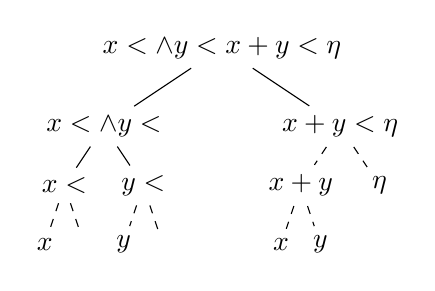
\begin{tikzpicture}
    \node (m) at (0,0) {$x<\eps\land y<\eps\implies x+y<\eta$};
    \node (l) at (-1.5,-1) {$x<\eps\land y<\eps$};
    \node (ll) at (-2,-1.75) {$x<\eps$};
    \node (lll) at (-2.25,-2.5) {$x$};
    \node (llr) at (-1.75,-2.5) {$\eps$};
    \node (lr) at (-1,-1.75) {$y<\eps$};
    \node (lrl) at (-1.25,-2.5) {$y$};
    \node (lrr) at (-0.75,-2.5) {$\eps$};
    \node (r) at (1.5,-1) {$x+y<\eta$};
    \node (rl) at (1,-1.75) {$x+y$};
    \node (rll) at (0.75,-2.5) {$x$};
    \node (rlr) at (1.25,-2.5) {$y$};
    \node (rr) at (2,-1.75) {$\eta$};

    \draw (m) -- (l) -- (ll);
    \draw (l) -- (lr);
    \draw (m) -- (r);

    \draw [dashed] (ll) -- (lll);
    \draw [dashed] (ll) -- (llr);
    \draw [dashed] (lr) -- (lrl);
    \draw [dashed] (lr) -- (lrr);

    \draw [dashed] (r) -- (rl) -- (rll);
    \draw [dashed] (rl) -- (rlr);
    \draw [dashed] (r) -- (rr);
  \end{tikzpicture}

  \caption{Разложение формулы до переменных}\label{fig:form_var}
\end{marginfigure}

{\it Константа}\index{константа} --- $0$-арный
функциональный или предикатный знак.
% Если $\psi$ --- $n$-арный функциональный или предикатный знак, то в выражении
% $\psi(t_1,...,t_{n})$ термы $t_1,...,t_{n}$ называют
% {\it аргументами}
% $\psi$.

Аналогично с формулами можно рассматривать и деревья термов.
Формулы можно разложить до элементарных формул. Элементарные формулы
можно разложить на термы. Термы можно разложить до переменных (рис.~\ref{fig:form_var}).

При интерпретации формул термы соответствуют объектам, а формулы --- высказываниям
об этих объектах. Объекты, которым соответствуют термы определяются изучаемой
областью математики. Например, в теории множеств всякий терм --- множество.

\section{Кванторы}

Добавим в язык возмножность формулировать утверждения о существовании
какого-то объекта и о всеобщности какого-то свойства для всех рассматриваемых объектов.
Введём в алфавит союзы $\forall$
--- {\it квантор всеобщности}\index{квантор!всеобщности} и $\exists$
--- {\it квантор существования}\index{квантор!существования}.

\pagebreak
Будем говорить, что
\begin{enumerate}
  \index{связанная переменная}\index{переменная!связанная}
  \item{}Переменная $\gamma$ {\it связанна}
  в формуле $F$, если $F$ содержит
  выражение $K\gamma$, где $K$~---~квантор.

  \index{свободная переменная}\index{переменная!свободная}
  \item{}Переменная $\gamma$ {\it свободна}
  в формуле $F$, если $F$ содержит $\gamma$,
  но $\gamma$ не связанна в $F$.

  \index{формула!о переменной}
  \item{}$F$ --- {\it формула о переменной} $\gamma$, если $\gamma$
  не связанна в формуле $F$.
  То есть либо $F$ не содержит $\gamma$, либо $\gamma$ свободна в $F$.

  \index{формула!замкнутая}\index{замкнутая формула}
  \item{}{\it Замкнутая формула} --- формула без свободных переменных.
\end{enumerate}

Например, $F\equiv x=2$ --- формула о $x$ и $x$ свободна в $F$.
Заметим, что формула $F$ также является формулой об $y$, причём $F$ не содержит $y$.

Расширим понятие формулы:
Если $F$ --- формула о $x$, то выражения $(\forall x)~F$, $\exists x:F$
также являются формулами.

Формула $(\forall x)F$ соответствует высказыванию
``$F$ для всякого (произвольного, любого) $x$''.
Формула $\exists x:F$ соотвествуют высказыванию
``Существует такой $x$, что $F$''.

Определим алгоритм разложения сложной формулы.
Пусть $K$~---~квантор, $\gamma$ --- переменная.
\begin{enumerate}
  \item{}Если формула начинается с $K\gamma$, то разлагаем формулу по $K\gamma$.
  \item{}Далее в порядке
  \begin{multicols}{2}
    \begin{enumerate}
      \item{}$\implies$ или $\iff$.
      \item{}Самый правый $\lor$.
      \item{}Самый правый $\land$.
      \item{}Самый левый $\lnot$ или $K\gamma$.
    \end{enumerate}
  \end{multicols}
\end{enumerate}

\begin{marginfigure}[-4cm]
  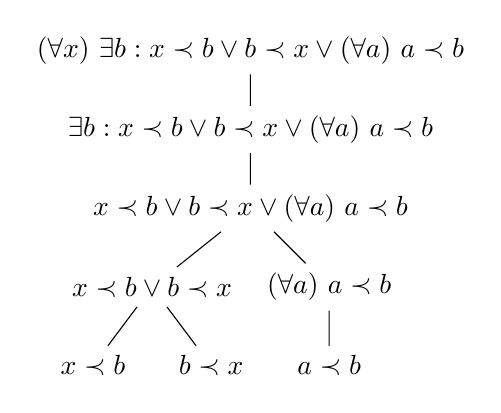
\begin{tikzpicture}
    \node (m) at (0,0) {$(\forall x)~\exists b:x\prec b\lor b\prec x
        \lor (\forall a)~a\prec b$};
    \node (mm) at (0,-1) {$\exists b:x\prec b\lor b\prec x
        \lor (\forall a)~a\prec b$};
    \node (mmm) at (0,-2) {$x\prec b\lor b\prec x\lor (\forall a)~a\prec b$};
    \node (mmmr) at (1,-3) {$(\forall a)~a\prec b$};
    \node (mmmrm) at (1,-4) {$a\prec b$};
    \node (mmml) at (-1.25,-3) {$x\prec b\lor b\prec x$};
    \node (mmmll) at (-2,-4) {$x\prec b$};
    \node (mmmlr) at (-0.5,-4) {$b\prec x$};

    \draw (m) -- (mm) -- (mmm) -- (mmmr) -- (mmmrm);
    \draw (mmm) -- (mmml) -- (mmmll);
    \draw (mmml) -- (mmmlr);
  \end{tikzpicture}

  \caption{Дерево более сложной формулы.}\label{fig:comp_tree}
\end{marginfigure}

Пусть $\prec$ --- бинарный предикатный знак.
На рис.~\ref{fig:comp_tree} представлен пример разложения более
сложной формулы в дерево.

Часто формулы с кванторами сокращают:
\begin{enumerate}
  \item{}$(\forall x:Q)~R\equiv (\forall x)~Q\implies R$

  $(\forall x:Q)~R$ соответствует ``$R$ для всякого $x$ такого, что $Q$''.

  \item{}$(\forall x\prec a)~P\equiv (\forall x:x\prec a)~P$,
  где $\prec$ --- любой бинарный предикатный знак.

  ${(\forall x\prec a)~P}$ соотвествует
  ``$P$ для всякого $x\prec a$''.

  \item{}$\exists x\prec a:P\equiv\exists x:x\prec a\land P$

  $\exists x\prec a:P$ соотвествует
  ``Существует такой $x\prec a$, что $P$''.

  \item{}Части с одинаковыми кванторами можно объединить:
  \[
    (\forall x,y)~P\equiv(\forall x)(\forall y)~P\qquad
    \exists x,y:P\equiv\exists x:\exists y:P
  \]

  \item{}Правила 2,3,4 можно объединить:
  \[
    \begin{aligned}
       & (\forall x_{11},...,x_{1k_1}\zeta_1a_1,x_{21},...,x_{2k_2}\zeta_2a_2,...,
      x_{n1},...,x_{nk_n}\zeta_na_n,y_1,...,y_{m})~P\equiv                         \\
       & \equiv (\forall x_{11}\zeta_{1}a_1)...(\forall x_{1k_1}\zeta_1a_1)...
      (\forall x_{n1}\zeta_{n}a_{n})...(\forall x_{nk_{n}}\zeta_{n}a_{n})
      (\forall y_1)...(\forall y_{m})~P
    \end{aligned}
  \]
  Например,
  \[
    (\forall x,y\leq 0,n>1,u,v)~P\equiv (\forall x\leq 0)(\forall y\leq 0)
    (\forall n>1)(\forall u)(\forall v)~P
  \]
  Аналогично с $\exists$.

  \item{}Некоторые авторы опускают ``$:$'' после $\exists$ и
  ставят выражение $\exists x$ в скобки:
  $(\exists x)P\equiv \exists x:P$.

  \item{}Скобки вокруг $\forall x$ или $\exists x$ можно опустить,
  если после него следует квантор или выражение в скобках.
  То есть
  \[
    \forall y\forall x (x=x)\equiv (\forall y)(\forall x)(x=x)\qquad
    \exists y\exists x(x=x)\equiv (\exists y)(\exists x)(x=x)
  \]
\end{enumerate}

Например, формулу
\newcommand\N{\mathbb N}
\begin{equation}\label{eq:nat_unbound}
  (\forall r)~r\in\N\implies \exists n:n\in\N\land n>r,
\end{equation}
где $x\in\N$ тогда и только тогда, когда $x$ --- натуральное число, можно записать как
\[
  \forall r\in\N~\exists n\in\N:n>r\quad\text{или}\quad
  (\forall r\in\N)(\exists n\in\N)~n>r
\]
Эти формулы соотвествуют ``Для произвольного натурального числа
$r$ существует такое натуральное $n$, что $n>r$''.

Для кванторов выполняются (являются истинными формулами)\footnote{
  На данный момент мы не можем их доказать, а только
  обосновать словесными рассуждениями.

  На данный момент мы ничего не можем доказать, потому что мы не ввели
  понятие доказуемости.}
следующие {\it законы отрицания}\index{закон!отрицания кванторов}:
\[
  \lnot[(\forall x)~P]\iff[\exists x:\lnot P]\qquad
  \lnot[\exists x:P]\iff[(\forall x)~\lnot P]
\]

Если переменная $\gamma$ связанна в формуле $F$, то её буква не имеет значения.
Например, следующие две формулы эквивалентны:
\[
  (\forall p)~(p>0\implies p \geq 0)\qquad
  (\forall \chi)~(\chi>0\implies \chi\geq 0)
\]

Введём обозначение для замены знаков в выражениях.
Возьмём выражение $P$, заменим в нём все выражения $\alpha$ выражением $\beta$ и
обозначим полученное выражение как $P(\beta/\alpha)$, что читают как
``$P$ $\beta$ вместо $\alpha$''.
Если мы заменяем не все $\alpha$ выражением $\beta$, то можем обозначить полученное
выражение как $P(\beta/'\alpha)$.
Например, если $Q\equiv x+y=2y$, то $Q(t/y)\equiv x+t=2t$ и $Q(t/'y)$ может
обозначать любое из выражений
\[
  x+y=2y\qquad x+t=2y\qquad x+y=2t\qquad x+t=2t
\]

Если $P$ --- формула о $x$, то часто вводят обозначения
\[
  P(x)\equiv P\qquad P(t)\equiv P(t/x)
\]

Если одна переменная связанна в двух разных подформулах
одной формулы, то эти два использования
одного знака не имеют друг к другу никакого отношения.
Например, следующие две формулы эквивалентны:
\[
  [(\forall x)~P(x)]\land[\exists x:Q(x)]\qquad
  [(\forall \alpha)~P(\alpha)]\land[\exists \beta:Q(\beta)],
\]

\phantomsection{}\label{page:exists_only}
Если в языке введён бинарный предикатный знак $=$, то
можем определить сокращения
\[
  \exists! x:P(x)\equiv[\exists x:P(x)]\land
  [(\forall x,y)~P(x)\land P(y)\implies x=y]
\]
\[
  \exists! x\prec a:P(x)\equiv \exists! x:x\prec a\land P(x),
\]
где знак $\exists!$ --- {\it квантор существования и единственности}.
\index{квантор!существования!и единственности}

\vspace{1em}
{\it Упражнения:}
\begin{enumerate}
  \item{}Обосновать на основе словесных рассуждений законы отрицания
  кванторов\label{ex:quantor_neg_def}. Вывести законы отрицания формул
  $p\land q$ и $p\lor q$, заметить схожесть с законами отрицания кванторов.
  В чём по смыслу схожи $\land$ и $\forall$? $\lor$ и $\exists$?

  \item{}Разложить в дерево формулу \eqref{eq:nat_unbound}.

  \item{}Упростить формулы
  \begin{multicols}{2}
    \begin{enumerate}
      \item{}$\lnot[\forall x~\exists y:P(x,y)]$
      \item{}$\lnot[(\forall x)~ x\prec a\land P(x)]$
      \item{}$\lnot[(\forall x\prec a)~P(x)]$
      \item{}$\lnot[\exists x\prec a:P(x)]$
    \end{enumerate}
  \end{multicols}
  пользуясь законами отрицания кванторов.
  Например,
  \[
    \lnot [(\forall x)(\forall y)~P]\quad\to\quad
    \exists x:\lnot [(\forall y)~P]\quad\to\quad
    \exists x:\exists y:\lnot P
  \]
  Для удобства обозначим $x\nprec a\equiv \lnot(x\prec a)$.

  \item{}Обосновать условие единственности:
  \[
    (\forall x,y)~P(x)\land P(y)\implies x=y
  \]
\end{enumerate}
